\section{Usability Test Results}
\label{sec:usabilityresults}
In order to protect the identity of our test subjects, especially considering the children, we have used identifiers as names. Names starting with the letter ``A'' is an adult user, and names starting with ``C'' denotes a child.

As mentioned in Chapter \ref{sec:testmethod}, the problems discovered were rated according to the severity. These errors can be found under the header \emph{Level} in the respective tables. To recap, the ranking goes as follows: Level 1 is a critical error, Level 2 is a significant problem with accomplishing a task, Level 3 is a minor issue with the usability and Level 4 is non-essential issue. 
  

\subsection{Parent Partition Tests}

\subsubsection{Adult User 1}
\begin{table}[H]
\centering
\begin{tabular}{|p{4.0cm} | p{4.0cm} |}
	\hline
	\textbf{Name} & AU1\\
	\hline
	\textbf{Age} & 36 \\
	\hline
	\textbf{Gender} & Male \\
 	\hline 
	\textbf{Date} & May 2nd, 2014 \\
	\hline
	\textbf{Testleader} & Aleksander\\
	\hline
	\textbf{Observer} & Esben\\
	\hline	
\end{tabular}
\end{table}

\begin{singlespacing}
\begin{table}[H]
\centering
\begin{tabular}{| p{0.7cm} | p{4.0cm} | p{0.9cm} | p{3.7cm} | p{3.3cm} |}
\hline
	\textbf{Task} & \textbf{Problem} & \textbf{Level} & \textbf{Cause} & \textbf{Proposal for solution} \\
	\hline
	0 & The user where unable to separate between the image for child and parent partition. & 3 & The images were not entirely intuitive. & The image for adults could have a bearded man, or other recognizable features. \\
	\hline
	1 & It was unclear whether he had to press on the healthy medicine plan, as the child was in the healthy medicine plan by default. & 3 & Challenging GUI. & Could make it clearer for the user which treatment plan is being followed. \\
	\hline
	1 & The spinners for hour/minutes should be able to be written into. & 3 & The standard Android slider contains a minor bug when one writes into it.  & N/A \\
	\hline
	1 & The timestamp contained seconds, which caused annoyance. & 4 & Timestamp contains seconds. & Remove seconds from the timestamp. \\
	\hline
	2 & The user expected that he could press the medicine, and not just the checkbox which was the case. He found this a little annoying. & 3 & Implementation of listener. & Make the entire list item touchable. \\
	\hline
	2 & He wanted functionality for adding two medicines at once. & 2 & This has not been implemented yet. & Implement it later. \\
	\hline
	3 & The view shows a button with ``Add Activity'', which he felt was wrong. & 3 & This was not intended, as it should have said ``Add Reward''. & Change it to ``Add Reward''. \\
	\hline
	3 & When pressing the back button one too many times, he was challenged with the PIN code again. This caused annoyance. & 4 & PIN-challenge appears as soon a parent returns from the parent partition. & Could implement a timer who checks when the user last completed the challenge.\\
	\hline
	4 & The test user said it was not logical to see where he could check the air quality cast. & 3 & Bad task description. & Change task description to make it more understandable. \\
	\hline
	4 & The test user wanted functionality for different views, for instance showing the log for a week or a single day. & 4 & Confusing calendar view. & This feature could be implemented with more time and resources.  \\
	\hline
\end{tabular}
\caption{Usability Test Results: AU1}
\label{tab:testadult1}
\end{table}
\end{singlespacing}


\subsubsection{Adult User 2}

\begin{table}[H]
\centering
\begin{tabular}{| p{4.0cm} | p{4.0cm} |}
\hline
 \textbf{Name} & AU2 \\
 \hline
 \textbf{Age} & 35 years old \\
 \hline 
 \textbf{Gender} & Male \\
 \hline 
 \textbf{Date} & May 7th, 2014 \\
 \hline
 \textbf{Testleader} & Aleksander \\
 \hline
 \textbf{Observer} & Esben \\
 \hline
\end{tabular}
\end{table}

\begin{singlespacing}
\begin{table}[H]
\centering
\begin{tabular}{| p{0.8cm} | p{2.8cm} | p{0.9cm} | p{5.0cm} | p{3.1cm} |}
\hline
	\textbf{Task} & \textbf{Problem} & \textbf{Level} & \textbf{Cause} & \textbf{Proposal for solution} \\
	\hline
	2 & The user did not know whether the alarm should fire at a given time or if the child should actually take the medicine at that time. & 2 & The view only prompts the user to insert a time. & Could change the text ``Time'' to ``Time the alarm should trigger'', or similar. \\
	\hline
	2 & Alarms were not added properly. & 1 & Discovered a bug; When the user opens the application for the first time, it adds a user to the database. As the device was not connected to any network, this failed, and we had not implemented feedback to the user. & Implement the functionality needed, and give feedback to the user. \\
	\hline
	3 & The user did not know whether he had actually selected an image. & 2 & The ``Add Reward'' module does not provide enough feedback as to whether or not the user has actually selected an image. & This functionality should be implemented.  \\
	\hline
	3 & The user did not understand what repeat meant. & 3 & Repeat means to give the same reward on a continuous basis, for the same amount of stars given. This was not explained well enough on the user test. & Clarify this aspect with a help box.   \\
	\hline
	5 & The air quality cast does not change with regards to which day is picked. & 3 & The air quality is currently only imported for the current date. & \app{} should give feedback that the queried data is not available for days later than today. \\ 
	\hline
	5 & The user was confused when deciding which day was selected. & 2 & The view does not provide enough feedback to ensure the user of which day is selected. & Implementation of the feature could be performed. Additionally, we could add separate views to show a week or a day, and not only showing the month. \\
	\hline  
\end{tabular}
\caption{Usability Test Results: AU1}
\label{tab:testadult2}
\end{table}
\end{singlespacing}


\textbf{Comments about the test}

The execution of this user test unfortunately suffered from a mistake made before initiating the test. When we started it, the Android device were not connected to the network. As such, task 2 uncovered a bug that we had never seen before. In order to get any useful testing started, we had to reset the application and connect it to the network, before we started over again. The first impression was probably not the best.   


\subsection{Child Partition}
\label{sec:childresults}

During the user tests, \ab{} was configured to use the varied interaction scheme. This involved a preset combination of the remaining interactions from Table \ref{tab:interactioneval}. This decision was made in order to test all of the possible interactions, as we did not have enough users to test them one-by-one. 

\subsubsection{Child User 1}
\begin{table}[H]
\centering
\begin{tabular}{| p{4.0cm} | p{4.0cm} |}
\hline
 \textbf{Name} & CU1 \\
 \hline
 \textbf{Age} & 6 years old \\
 \hline 
 \textbf{Gender} & Female \\
 \hline 
 \textbf{Date} & May 2nd, 2014 \\
 \hline
 \textbf{Testleader} & Aleksander \\
 \hline
 \textbf{Observer} & Esben \\
 \hline
\end{tabular}
\end{table}

\begin{table}[H]
\centering
\begin{tabular}{| p{1.0cm} | p{4.0cm} | p{0.9cm} | p{3.6cm} | p{3.1cm} |}
\hline
	\textbf{Task} & \textbf{Problem} & \textbf{Level} & \textbf{Cause} & \textbf{Proposal for solution} \\
	\hline
	2 & It seemed like she had a hard time keeping up with \ab{}'s instructions & 2 & The voice of \ab{} was speaking to fast & Record sounds with lower speed \\
	\hline
	4 & It was difficult to drag the medicine above the mask in order to start the treatment & 3 & The treatment only starts when the medicine is directly above the mask & Should make this functionality simpler to start.  \\
	\hline
	4 & It was hard for the child to keep ut with the voice of the rabbit. & 2 & The voice talked to quickly, and \app{} does not have a repeat functionality when a treatment is running. & Should consider implementing repeat.\\ 
	\hline
	5 & It was hard to get a clean read of the RFID tag. & 3 & It was not entirely clear where the user had to put the card in order to get a read. & \ab{} should have an indicator as of where the card should be held in order to be read.  \\
	\hline
\end{tabular}
\caption{Usability Test Results: CU1}
\label{tab:testchild1}
\end{table}

\textbf{Comments about the test}

CU1 was very shy when arriving at the test lab. It quickly became clear for us that we had to leave the area and rather observe from the back room, in order for her to speak up. The parent was instructed with the tasks that were to be performed, and he explained the tasks to her. Once we were back stage, she started responding to the instructions given. We made a note that the observer should sit in the back room and observe from there, in order for the children to respond more easily.   

When asked which method CU1 preferred, i.e. \app{} or \ab{}, CU1 replied ``I don't know''. CU1 was also asked if both were equally fun, which to CU1 replied ``Yes''. CU1 was also asked if the usage of \app{} and \ab{} was more fun than a regular treatment, which to CU replied ``Yes''\footnote{There is reason to believe that the answer was biased due to the reward}. We asked if this was because of her reward, which was candy, but we were unable to get a reply. 

\subsubsection{Child User 2}
%Personalia user 2
\begin{table}[H]
\centering
\begin{tabular}{| p{4.0cm} | p{4.0cm} |}
\hline
 \textbf{Name} & CU2 \\
 \hline
 \textbf{Age} & 7 years old \\
 \hline 
 \textbf{Gender} & Male \\
 \hline
 \textbf{Date} & May 2nd, 2014 \\
 \hline
 \textbf{Testleader} & Aleksander \\
 \hline
 \textbf{Observer} & Esben \\
 \hline
\end{tabular}
\end{table}

\begin{table}[H]
\centering
\begin{tabular}{| p{1.0cm} | p{4.0cm} | p{0.9cm} | p{3.1cm} | p{3.7cm} |}
\hline
	\textbf{Task} & \textbf{Problem} & \textbf{Level} & \textbf{Cause} & \textbf{Proposal for solution} \\
	\hline
	2 & The user did not know whether he should hold the medicine or the mask towards the mouth. & N/A & We believe this falls under the category of human errors, as he may weren't able to distinguish between the two. & The voice instruction could put more emphasis on \emph{medicine}. \\
	\hline
	2 & When the user was supposed to count to 10, he counted too fast, leaving \ab{} to breathe for several seconds after he had finished counting. & 3 & He may not be aware of how long time a second takes. & The light on \ab{}'s nose could light only when he is supposed to count. \\
	\hline
\end{tabular}
\caption{Usability Test Results: CU2}
\label{tab:testchild2}
\end{table}

\begin{figure}
	\begin{minipage}[t]{0.4\linewidth}
		\centering
			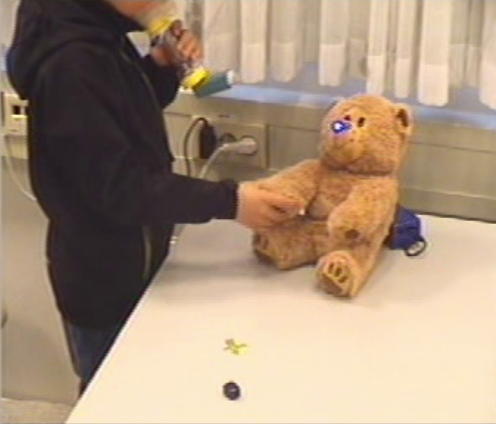
\includegraphics[width=0.30\paperwidth]{Pictures/usability-pictures/CU2-interacting.png}
		\label{fig:child-interacting-while-breathing}
		\caption[CU2 interacting with \ab{}]{CU2 interacting with \ab{} while taking his medicine}
	\end{minipage}
	\hspace{1.5cm}
	\begin{minipage}[t]{0.4\linewidth}
		\centering
			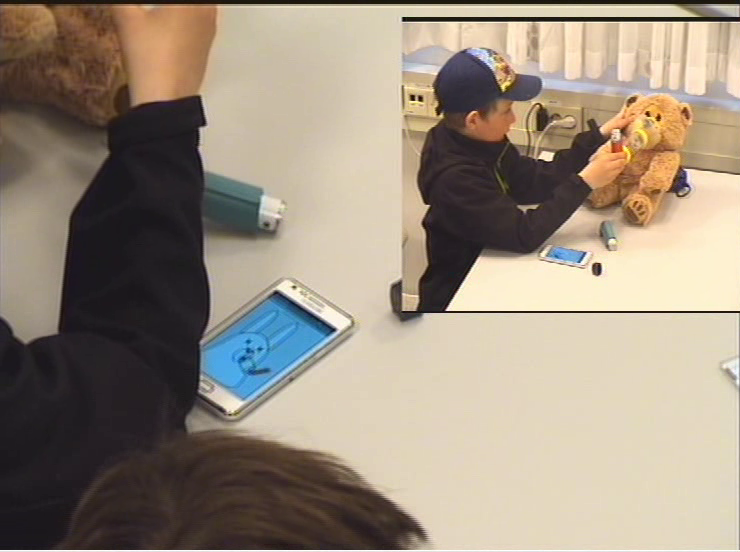
\includegraphics[width=0.30\paperwidth]{Pictures/usability-pictures/CU2-app.png}
		\label{fig:child-medicating-ab}
		\caption[CU2 giving \ab{} a medicine]{After having completed one treatment, CU2 decided to give \ab{} another round of medicine}
	\end{minipage}
\end{figure}

\textbf{Comments about the test}

When asked about which system he liked the most, CU2 first replied that he liked both systems equally. When we ``pushed'' him to pick one, he thought that \ab{} was more fun to interact with, as it had lights that blinked. He also liked \app{}, as it contained the store where he could buy a reward. 

\subsubsection{Child User 3}
%Personalia user 3
\begin{table}[H]
\centering
\begin{tabular}{| p{4.0cm} | p{4.0cm} |}
\hline
 \textbf{Name} & CU3 \\
 \hline
 \textbf{Age} & 5 years old \\
 \hline 
 \textbf{Gender} & Male \\
 \hline
 \textbf{Date} & May 7th, 2014 \\
 \hline
 \textbf{Testleader} & Aleksander \\
 \hline
 \textbf{Observer} & Esben \\
 \hline
\end{tabular}
\end{table}


\begin{table}[H]
\centering
\begin{tabular}{| p{1.0cm} | p{4.0cm} | p{0.9cm} | p{3.1cm} | p{3.5cm} |}
	\hline
	\textbf{Task} & \textbf{Problem} & \textbf{Level} & \textbf{Cause} & \textbf{Proposal for solution} \\
	\hline
	2 & The user did not understand whether he should clap his own hands or \ab{}'s. & 3 & The voice of \ab{} spoke to fast. & Record sounds that talks slower. \\
	\hline
	2 & When giving \ab{} a high five, he hit too hard, giving \ab{} a knock out. & 2 & \ab{} has a stability issue. & The high five interaction might only be suitable for more stable artefacts. \\
	\hline
	3 & The user did not know whether he should press \ab{}'s head or the animation on \app{}. & 4 & The user had both \ab{} and \app{} in front of him during the user tests. & This could easily be avoided by removing \ab{} from the scene when we switched tasks. \\
	\hline  
\end{tabular}
\caption{Usability Test Results: CU3}
\label{tab:testchild3}
\end{table}

\clearpage{}

\begin{figure}
	\begin{minipage}[t]{0.3\linewidth}
		\centering
			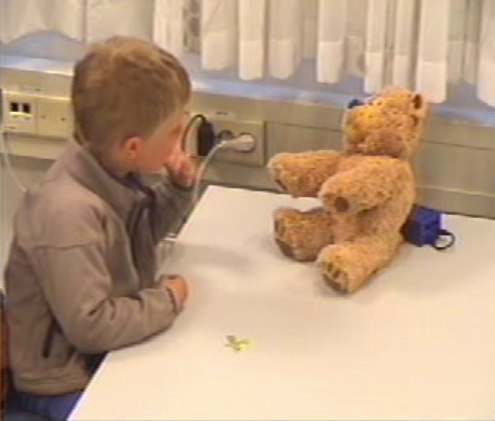
\includegraphics[width=0.20\paperwidth]{Pictures/usability-pictures/knockout1.png}
		\label{fig:child-knockout1}
	\end{minipage}
	\hspace{0.5cm}
	\begin{minipage}[t]{0.3\linewidth}
		\centering
			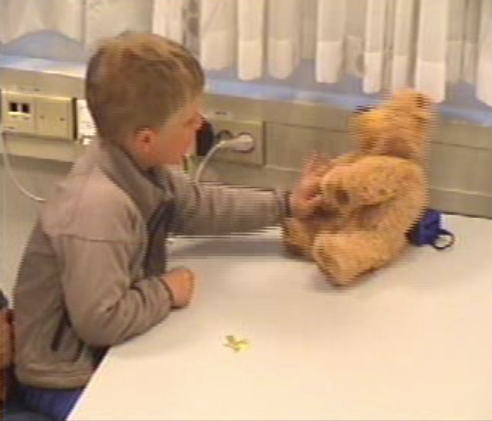
\includegraphics[width=0.20\paperwidth]{Pictures/usability-pictures/knockout2.png}
		\label{fig:child-knockout2}
	\end{minipage}
	\hspace{0.5cm}
	\begin{minipage}[t]{0.3\linewidth}
		\centering
			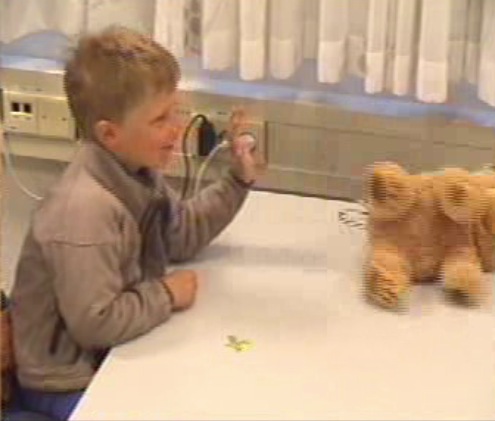
\includegraphics[width=0.20\paperwidth]{Pictures/usability-pictures/knockout3.png}
		\label{fig:child-knockout3}
	\end{minipage}
	\label{fig:child-knockout}
	\caption{CU3 knocks out \ab{} when giving him a high five}
\end{figure}

\textbf{Comments about the test}

When asked about which system he liked the most, CU3 switched back and forth between the \app{} and both. After analyzing the recordings, we found strong reason to believe that he had most fun when using \app{}. 


A problem not mentioned in Table \ref{tab:testchild3}, was that he was not able to read the text when he was to buy a reward. We have put a lot of effort into minimizing the reading ability required from the children, but at a certain point, some text is in required. An option for reducing the reading capabilities required at this stage, could be to prerecord potential rewards, but it required too much resources to do this, in addition to becoming unsustainable in the long run when parents are to give personalized rewards. An image of the view he had problems with is included in Figure \ref{fig:asthmapp-purchase}.   
 
\begin{figure}[H]
	\centering
	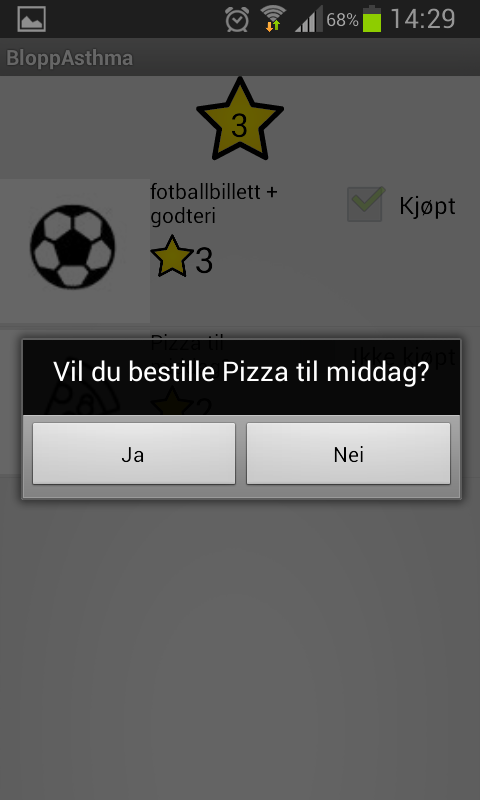
\includegraphics[width=0.25\paperwidth]{Pictures/app-screenshots/asthmapp-buy-screen.png}
	\caption{The view where CU3 had difficulties reading the information}
	\label{fig:asthmapp-purchase}
\end{figure}

